\chapter{The GEM and CSC Data Acquisition Systems}
\label{chap:II-2-daq}

  The installation of GEM detectors in CMS and the integration with the CSCs require the development of a new DAQ system for the GE1/1 project. The understanding of the structure of both the GEM and CSC readout chains as well as the common CMS central DAQ is of importance in the scope of this thesis. To this end, all three systems are presented in details in the sections that follow. \\

  \section{The GE1/1 Data Acquisition System}

    The architecture of the GE1/1 DAQ system is represented in Figure \ref{fig:II-2-daq-gem-system}. It is divided into two sectors: the on-detector electronics on the left in charge of the managment of the detector, and the off-detector electronics on the right responsable for the data handling and the connection to the central DAQ. The two sectors are separated by a few douzen meters and connected through optical fibres. \\

    \begin{figure}[h!]
      \centering
      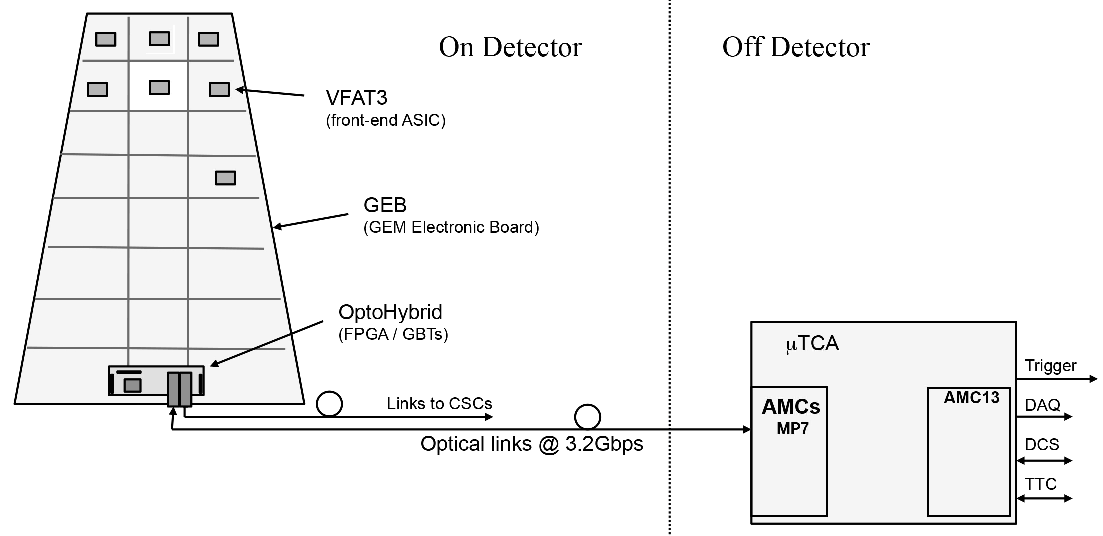
\includegraphics[width=0.7\textwidth]{img/II-2-daq/gem-system.pdf}
      \caption{??? \cite{Colaleo:2021453}.}
      \label{fig:II-2-daq-gem-system}
    \end{figure}

    The on-detector electronics focuses on the control and readout of the VFAT3 Application Specific Integrated Circuit (ASIC) which connects to the strips of the chamber and digitizes the data. The GEM Electronics Board (GEB), on which the VFAT3s are plugged in, then routes the signals to the OptoHybrid (OH) which acts as concentrator board and communication relay for the 24 VFAT3s. The communication with the off-detector system is performed through the GigaBit Tranciever (GBT) chipset and the Versatil Link installed on the OH. Both projects are led by CERN and provide radiation hard tools for LHC experiments. \\

    On the off-detector side, the Micro Telecommunications Computing Architecture (microTCA, MTCA, or $\mu$TCA) \cite{PICMG} crate standard is used to power and monitor the Advanced Mezzanine Cards (AMCs) which provide the ressources to communicate with the on-detector electronics. Links from multiple OHs are concentrated on one MP7 AMC which formats the data and transfers it to the CMS AMC13 mezzanine. The AMC13 is the link between the microTCA crate and the central DAQ of CMS which provides the clocking, trigger, and control over the system. The control of the DAQ chain is performed from a XDAQ application using the IPBus protocol over ethernet.

    \subsection{The VFAT3 ASIC}

      The VFAT3 ASIC is a binary front-end chip optimized for gaseous detectors which function is to digitize the analog signals coming from the detector and provide fast trigger and tracking data. The trigger data is sent at the LHC clock over a fixed latency path and then used in the algorithms of the L1 trigger to accept or reject events. The tracking data holds the full information on the events that have been accepted and follows a variable latency path. The logic diagram of the chip is shown in Figure \ref{fig:II-2-daq-vfat3}. It is made of an analog front-end which amplifies, shapes, and digitizes the signal from the GEM strips, and of a digital back-end for slow control and data readout. \\

      \begin{figure}[h!]
        \centering
        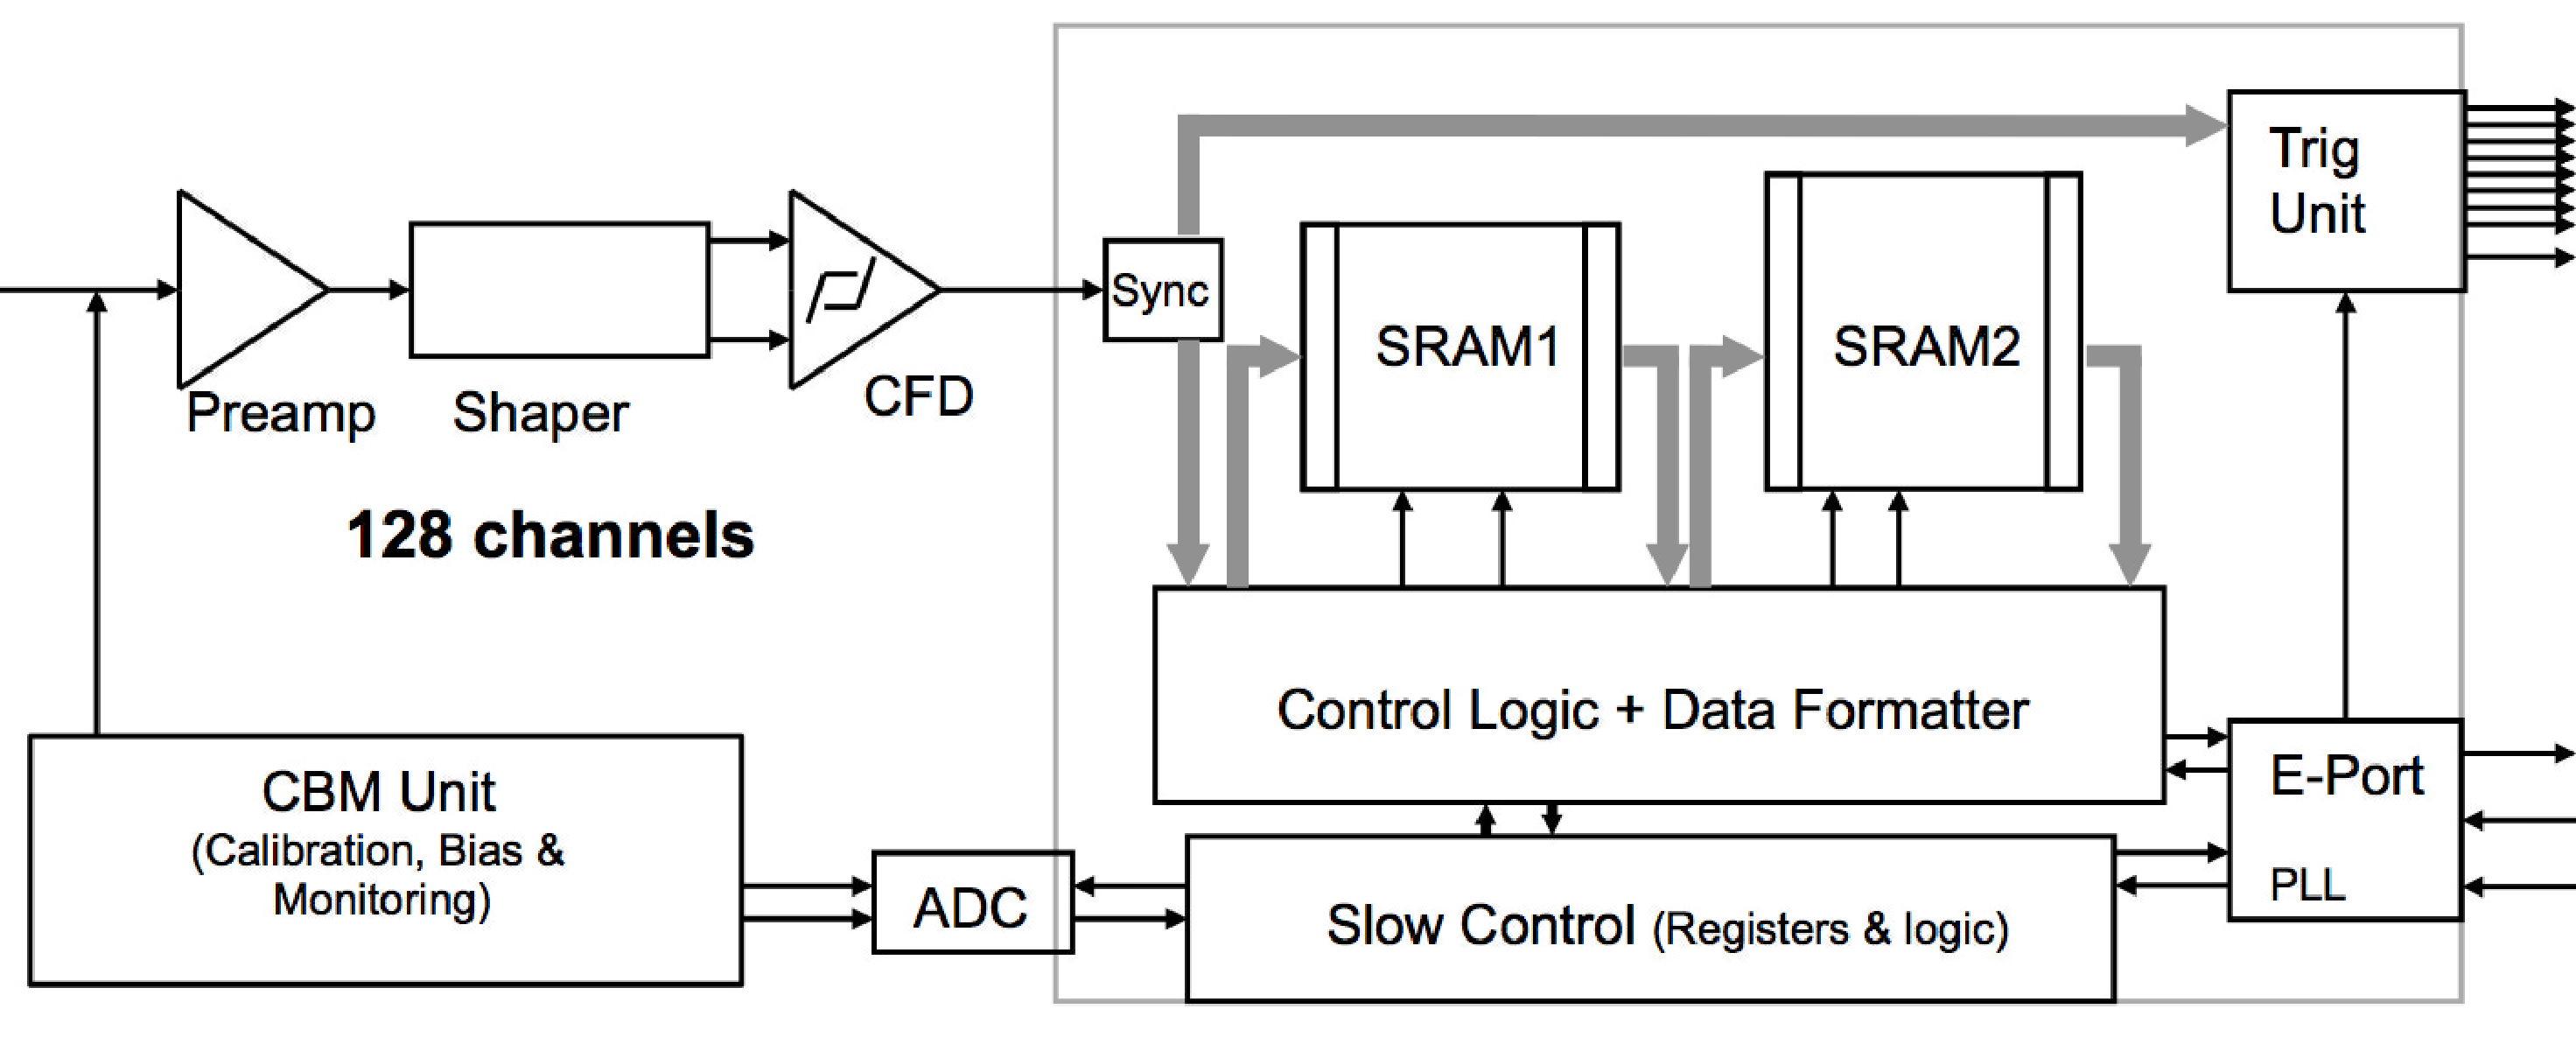
\includegraphics[width=\textwidth]{img/II-2-daq/vfat3.pdf}
        \caption{??? \cite{Colaleo:2021453}.}
        \label{fig:II-2-daq-vfat3}
      \end{figure}

      \paragraph{The analog front-end} is further optimized for the readout of GEMs in particular. It is composed of 128 channels which amplify and shape the analog signals from the strips with programmable shaping times to allow for various integration lengths of the signal. According to the gas mixture, signal charge from the GEM can last for approximatly 60 ns. Increasing the shaping time to fully integrate the charge will result in a higher signal to noise ratio. Simulations performed on the analog front-end show that a time resolution of 7 ns can be achieved by using a Constant Fraction Discriminator (CFD) with a shaping time of 50 ns. After shaping, the amplitude of the analog signal is compared against a programmable threshold by a comparator to yield a binary output flag. \\

      \paragraph{The fixed latency path} is used to provide a fast hit information to the trigger system of CMS at a frequency equal to the LHC clock of 40 MHz. The trigger unit inside the VFAT3 formats the results of the comparator and transmits it over 8 differential pairs at a rate of 64 bits per BX. It allows to either encode a logical-OR of two adjacent strips effectivly dividing the number of bits to send by a factor two, or use a zero supression algorithm to solely transmit information on hit strips. Ensuring a fixed latency on this path in crucial to maintain predictability in the trigger system and identify the correct BX. \\

      \paragraph{The variable latency path} is activated upon reception of an L1A to transmit the full granularity information on an event that has been accepted by the trigger system. The VFAT3 holds two Static Random-Access Memories (SRAMs) which are used to store events. The SRAM1 is a circular buffer filled at a frequency equal to the LHC clock with the output of the 128 comparators. When the VFAT3 receives an L1A, it transfers a given event from the SRAM1 to the SRAM2 and adds the BX Counter (BC) and the Event Counter (EC), which respectivly count the number of BX elapsed and the number of L1A received, to the event data. To determine which events needs to be transfered, the chip uses a programmable parameter called the latency that informs the system on the delay between the digitization of an event and the arrival of an L1A corresponding to the same event. It is a measures of the response time of the trigger system to a given event which is a fixed delay. Events stored in the SRAM2 are then formated and sent over a single differential pair out of the VFAT3. The formatting of the data can be selected using a programmable register to be either lossless or zero suppressed. \\

      \paragraph{The slow control} module handles the configuration of the internal registers of the VFAT3. These registers define quantities such as the threshold of the analog front-end, the latency, the readout data format, etc. Coupled with the Calibration, Bias \& Monitoring (CBM) unit, it allows to perform calibration routines on the chip. \\

      \paragraph{The fast control} defines all the time sensitive commands that the VFAT3 receives. These are the Event Counter 0 (EC0), Bunch Counter 0 (BC0), Calibration Pulse (CalPulse), Resynchronisation (Resync), and L1A. The EC0 and BC0 commands respectivly reset the EC and BC; the CalPulse is used to send a calibration pulse on given strips in order to callibrate the analog front-end; the ReSync command resets the EC counter; and the L1A informs the VFAT3 that an event needs to be transfered to the DAQ.

    \subsection{The GEM Electronics Board}

    \subsection{The OptoHybrid}

    \subsection{The GBT and Versatil Link}

    \subsection{The microTCA Standard}

    \subsection{The MP7 Advanced Mezzanine Card}

    \subsection{The AMC13}

    \subsection{The IPBus Protocol}

    \subsection{The XDAQ Application}

  \section{The CSC Data Acquisition System}

  \section{The CMS Central Data Acquisition System}
